\documentclass[tikz, border=1pt]{standalone}
\usepackage{tikz}
\usetikzlibrary{arrows.meta, positioning}
\usepackage{xcolor,colortbl}
% Define extra colors
\definecolor{darkgreen}{rgb}{0.0, 0.5, 0.0} % Define a darker green

\begin{document}

\begin{figure}
    \centering

    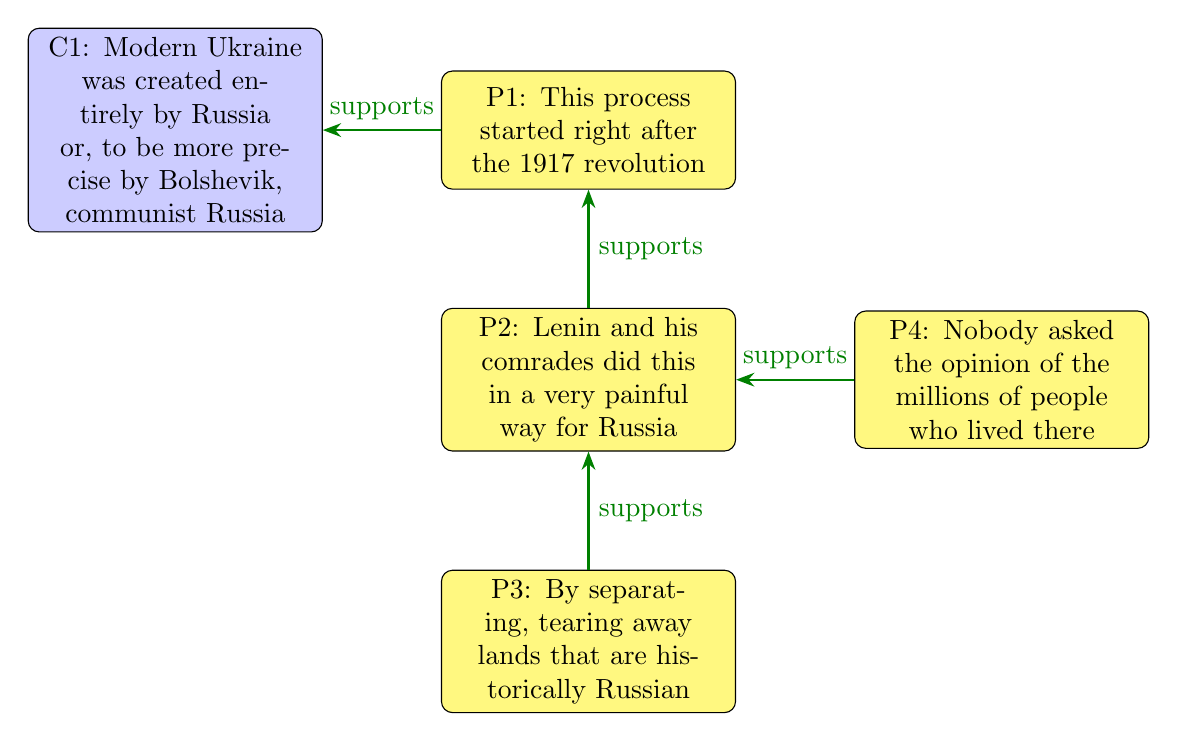
\begin{tikzpicture}[
        claim/.style={rectangle, draw, rounded corners, align=center, text width=3.5cm, minimum height=1.5cm, fill=blue!20},
        premise/.style={rectangle, draw, rounded corners, align=center, text width=3.5cm, minimum height=1.5cm, fill=yellow!50},
        arrow/.style={-{Stealth}, thick},
        support/.style={draw, -{Stealth}, thick, darkgreen},
        attack/.style={draw, -{Stealth}, thick, red},
        node distance=1.5cm and 1.5cm
        ]

        % Nodes
        \node (claim1) [claim] {C1: Modern Ukraine was created entirely by Russia or, to be more precise by Bolshevik, communist Russia};
        \node (premise1) [premise, right=of claim1] {P1: This process started right after the 1917 revolution};
        \node (premise2) [premise, below=of premise1] {P2: Lenin and his comrades did this in a very painful way for Russia};
        \node (premise3) [premise, below=of premise2] {P3: By separating, tearing away lands that are historically Russian};
        \node (premise4) [premise, right=of premise2] {P4: Nobody asked the opinion of the millions of people who lived there};

        % Arrows with labels
        \draw [support] (premise1) -- node[midway, above] {supports} (claim1);
        \draw [support] (premise2) -- node[midway, right] {supports} (premise1);
        \draw [support] (premise3) -- node[midway, right] {supports} (premise2);
        \draw [support] (premise4) -- node[midway, above] {supports} (premise2);

    \end{tikzpicture}
    % \caption{Argumentation structure for Example \ref{ex:legrandcontinent}}
    \label{fig:legrandcontinent}
\end{figure}

\end{document}